\chapter{Analysis}
\label{ch:analysis}
In the analysis
phase, the product requirements are derived --- defining the client expectations
for the product --- as well as the project constraints --- what the environments
limits about the product. Finally, the theoretical foundations are outlined,
providing the basic technical knowledge to undertake the project.

\section{Requirements}
\label{sec:requirements}
The requirements defined the client expectations for the TV remote control,
namely:
\begin{itemize}
\item Remotely operated
\item Low weight
\item Powered by batteries
\item 3 buttons: Power (Off/On); Up and Down for channel selection.
\item Infrared emitter response time (system output response time): 100 ms
\item The TV remote may be upgraded in the future to use more buttons
\end{itemize}

\section{Constraints}
\label{sec:constraints}
\begin{itemize}
\item Contains an infrared emitter (the TV already has an infrared receiver)
\item The TV remote control must supply the required data frames imposed by the TV
  manufacturer
\item Data frames may not be provided by the client
\item Security concerns are defined by the data frames and the specific
  communication frequency imposed by the TV manufacturer
\item 1 week deadline: 14 h
\item 2 people
\item Budget:
  \begin{itemize}
  \item HW (parts acquisition and assembly): fixed costs --- 1 EUR/unit
    \begin{itemize}
    \item TV remote Shell
    \item TV remote membrane
    \item Data acquisition \& Infrared emitter PCB
    \end{itemize}
  \item Development: project --- 20 EUR per hour per person, totalling 560 EUR +
    IVA
  \end{itemize}
\end{itemize}

\section{Theoretical foundations}
\label{sec:theor-found}
Pushing a button on a remote control sets in motion a series of events
that causes the controlled device to carry out a command. The process
works something like this:
\begin{enumerate}
\item 
Pushing the button on the remote control causes a touch to the contact beneath it and complete the button circuit on the circuit board. The integrated circuit detects this.
\item 
The integrated circuit sends the binary of the button function command to the LED at the front of the remote.
\item 
The LED sends out a series of light pulses that corresponds to the binary the button command.
\end{enumerate}
	

Here's an example of this clicking on the "volume up" button on a Sony TV Remote:

\begin{figure}
\centering
    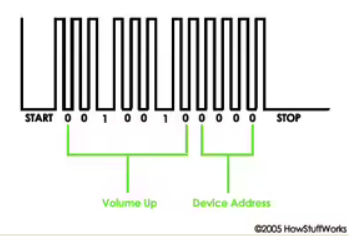
\includegraphics[width=0.5\columnwidth]{./img/buttoncode.png}
  \caption{Example of wave generator for "volume up" from~\cite{btncode})}%
\label{fig:btncode}
\end{figure}

The remote signal includes more than the command for "volume up". It sends
several bits of information to the receiving device, including:
\begin{itemize}
\item a "start" command
\item the command code for "volume up"
\item the device address (so the TV knows the data is intended for it)
\item a "stop" command (triggered when you release the "volume up" button)
\end{itemize}

In this case, the buttons that are needed and its codes are:

Power On = 001 0101

Power Off = 010 1111

Volume Up = 001 0010

Volume Down = 001 0011

%%% Local Variables:
%%% mode: latex
%%% TeX-master: "../../dissertation"
%%% End:
